%!TEX ROOT=DavidPetrDP.tex
\chapter{Ověření funkčnosti a možnosti využití přístroje}
Vzniklý FW měl fungovat s PC aplikací, která se již v používá společně STM32F042 v hodinách laboratoří průmyslové elektroniky(LPE), které se vyučují na ČVUT FEL a bylo tedy zapotřebí ověřit funkčnost všech implementovaných modulů. Funčnost nového firmware byla testována studenty již v průběhu letního semestru 2022/23, kdy tato práce vznikala. Současně funkci všech částí FW demonstruji v této kapitole prostřednictvím reálných záznamů běhu PC aplikace spolupracující s mým FW běžícím na mcu STM32G431
\section{Signálový Generátor}
\subsection{Rychlost přeběhu výstupního zesilovače DAC převodníku}
Maximální použitelná výstupní frekvence generátoru souvisí s omezenou rychlostí přeběhu(SR) výstupu DAC převodníku. Na obrázku \ref{fig:Obdelnik250kReal}, je vidět záznam měření, kdy jsem generoval obdélníkový signál s frekvencí 250KHz- tedy pouze 4 vzoky na periodu a byl zvolen v plný rozkmit výstupního signálu. Z obrázku je zřejmá omezená rychlost přeběhu, kterou můžeme rovnou změřit pomocí v aplikaci integrovaných kurzorů a dopočítat dle:
\begin{equation}
	\text{SR}=\frac{\Delta V}{\Delta t}=\frac{2.668 [\text{V}]}{1.387 [\mu\text{s}]}=1.92 [\text{V/}\mu\text{s}]
\end{equation}

Z tohoto je zřejmé, že rychlost přeběhu výstupního zesilovače je potřeba brát v potaz při volbě výstupní frekvence generovaného signálu a pokud potřebujeme generovat signál s vysokou výstupní frekvencí je dobré zvážit nižší rozkmit, aby signál nebyl tolik zkreslený.

\begin{figure}[H]
	\centering
	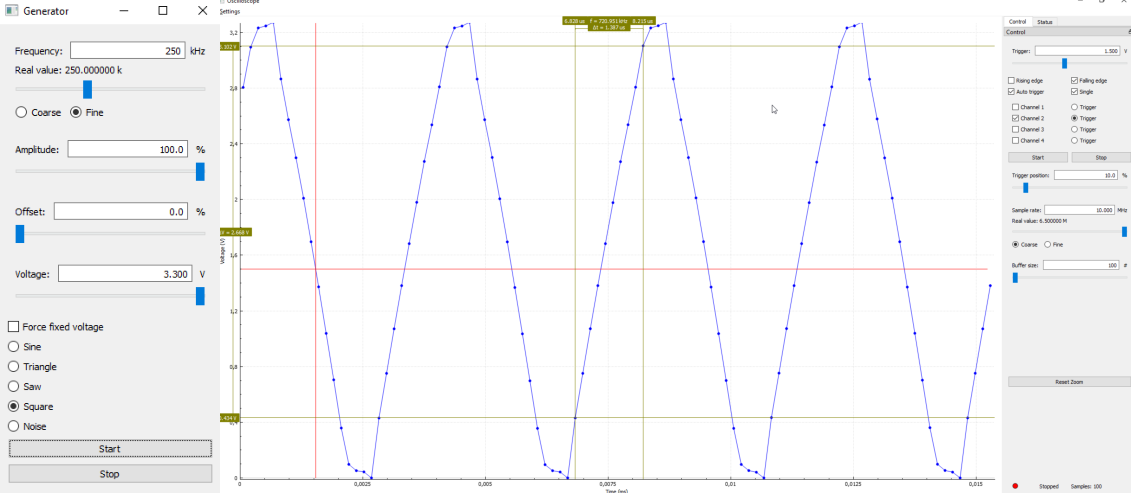
\includegraphics[width=0.9\linewidth]{Figs/Screenshots/RychlostPrebehuReal.pdf}
	\caption{Záznam obdélníkového signálu, $f_{\text{out}}$=250 kHz(4 vzorky na periodu) vzorkovaný rychlostí 6.5 MSps. Pozorování omezené rychlosti přeběhu výstupního zesilovače DAC převodníku}
	\label{fig:Obdelnik250kReal}
\end{figure}
\subsection{Vliv počtu vzorků an periodu}
V kapitole \ref{ch:signalGeneration} se zmiňuji o maximální vzorkovací frekvenci DAC převodníku a jeho vlivu na počet vzorků na periodu pro danou výstupní frekvenci signálu. Na obrázcích \ref{fig:sinus1000hz} a \ref{fig:sinus50khz} je vidět rozdíl v počtu vzorků na periodu při zvýšení výstupní frekvence signálu z 1000 Hz na 50 kHz
\begin{figure}[H]
	\centering
	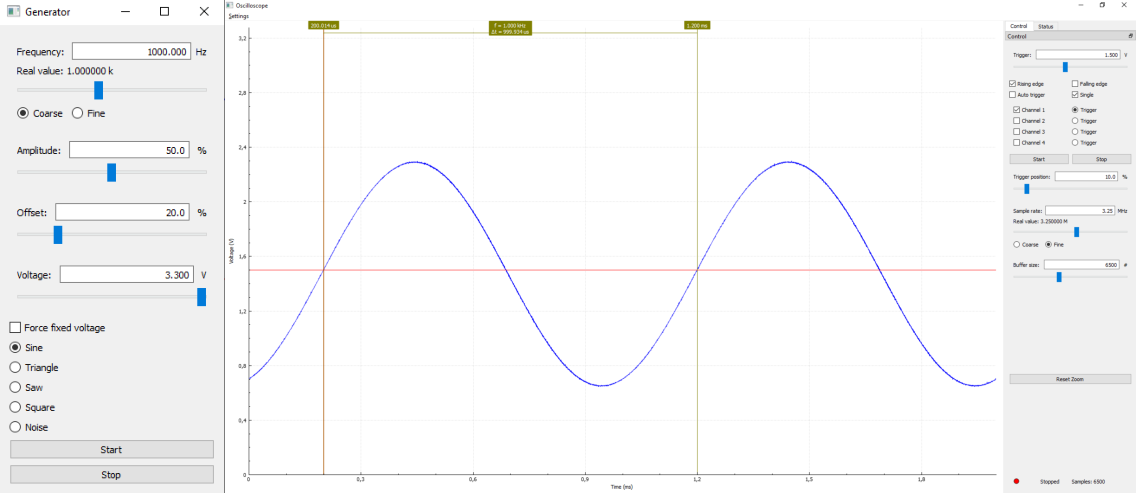
\includegraphics[width=0.9\linewidth]{Figs/Screenshots/Sinus1000Hz}
	\caption{Záznam signálu sinus o frekvenci 1000 Hz s 1000 vzorky na 1 periodu vzorkovaný rychlostí 3.25 Msps}
	\label{fig:sinus1000hz}
\end{figure}
\begin{figure}[H]
	\centering
	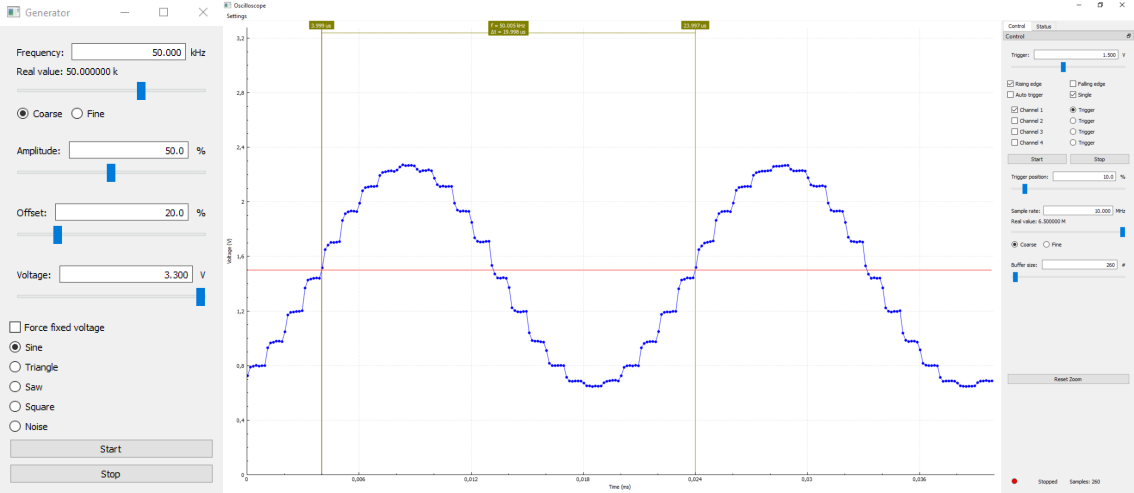
\includegraphics[width=0.9\linewidth]{Figs/Screenshots/Sine50K.pdf}
	\caption{Záznam signálu sinus o frekvenci 50 kHz s 20 vzorky na 1 periodu vzorkovaný rychlostí 6.5 Msps}
	\label{fig:sinus50khz}
\end{figure}

\section{Osciloskop}
\subsection{Ověření funkce v režimu ETS}
Aby bylo možné změřit přeběh použil jsem vzorkování v ekvivalentním vzorkování pro dosažení maximální vzorkovací frekvence 52 MSps. Tedy odečtený čas měření $\Delta T_{\text{SAMP}}$ je třeba nejdříve vhodně přepočíst koeficientem($k_{\text{AEQ}}$), abychom získali reálnou dobu přeběhu $\Delta T_{\text{SEQ}}$. Koeficient ($k_{\text{AEQ}}$) je závislý na frekvenci signálu $f_{\text{SIG}}=250$ kHz, frekvenci vzorkování $f_{\text{SAMP}}=9998.077$Hz a celočíselném koeficientu $k_s$.

\begin{equation}
	k_{\text{AEQ}}=\frac{f_{\text{SIG}}}{f_{\text{SIG}}-k_s\cdot f_{\text{SIG}}}, \quad k_s\approx\frac{f_{\text{SAMP}}}{f_{\text{SAMP}}}\approx\frac{250\text{kHz}}{9.998\text{kHz}}=25,\quad \Delta T_{\text{SEQ}}=\frac{\Delta T_{\text{SAMP}}}{k_{\text{AEQ}}}
\end{equation}

\begin{equation}
	k_{\text{AEQ}}=\frac{250\text{kHz}}{250\text{kHz}-25\cdot9.998\text{kHz}}=5200.208,\quad \Delta T_{\text{SEQ}}=\frac{7.112\text{ms}}{5200.208}
\end{equation}

\section{Logický analyzátor}

\section{Voltmetr se záznamem}
\begin{figure}[H]
	\centering
	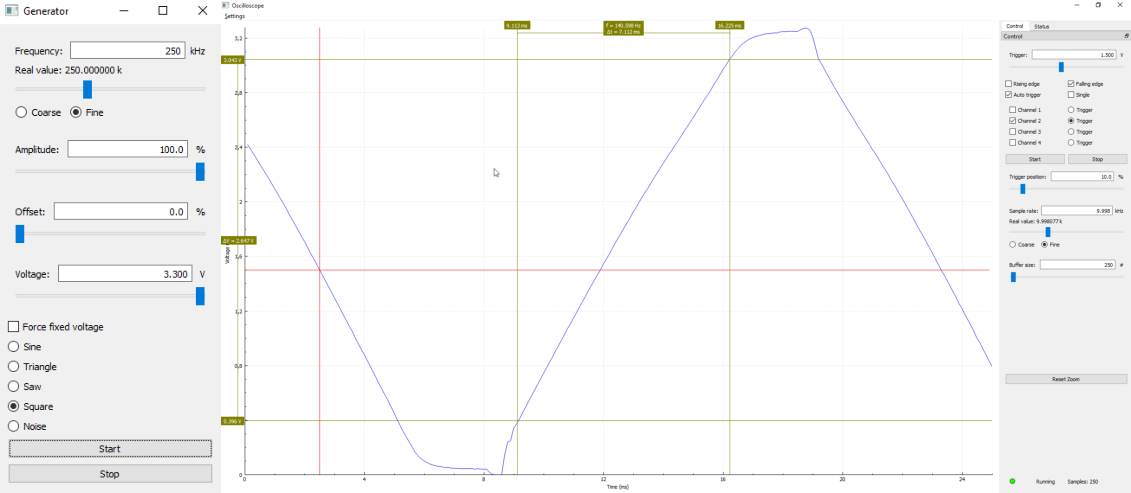
\includegraphics[width=0.9\linewidth]{Figs/Screenshots/RychlostPrebehu.pdf}
	\caption{Záznam voltmetru. Na kanálu č.1 signál sinus o frekvenci 1 Hz, Na kanálu č.2 PWM o frekvenci 2 Hz, Kanál č. 3 uzemněný}
	\label{fig:Voltmetr}
\end{figure}

\section{Čítač}

\begin{figure}[H]
	\centering
	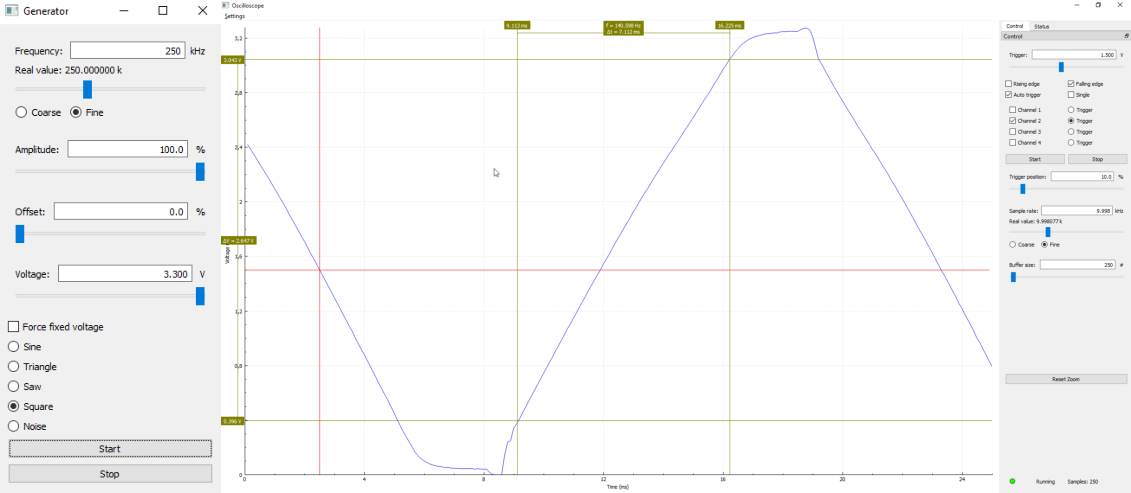
\includegraphics[width=0.9\linewidth]{Figs/Screenshots/RychlostPrebehu.pdf}
	\caption{Záznam signálu obdelník o frekvenci 250 kHz(4 vzorky) vzorkovaný rychlostí 52 Msps - omezeni rychlosti prebehu}
	\label{fig:Obdelnik250k}
\end{figure}



\section{Voltmetr se záznamem}
\subsection{Měření V-A charakteristiky}
\section{Aliasing}[H]
\newpage
\section{Parametry přístroje}
Pro budoucí referenci v této části shrnuji v této části dosažených parametrů přístroje s STM32G431.
\begin{itemize}
	\item \textbf{Základní vlastnosti}
	\begin{itemize}
		\item Frekvence systémových hodin a hodin čítačů - 156 MHz
		\item Frekvence hodin ADC převodníků - 52 MHz
		\item Možnost funkce pouze interním oscilátorem HSI nebo volitelně možnost připojit krystal s frekvencí 8 , 12 nebo 16 MHz
	\end{itemize}
	\item \textbf{Osciloskop}
	\begin{itemize}
		\item 4 kanály,záznam až 1x8192 vzorků(nebo 2x 4096, 4x 2048), rozlišení 12 bitů
		\item Rychlost záznamu až 1x 6.5 MS/s (nebo  2x 3.25 MS/s, 4 x 1.677 kS/s)
		\item Ve stroboskopickém módu - až  52 MS/s - rozlišení s intervalem 19,2 ns.
		\item Nastavení vzorkovací frekvence po 1Hz (1-9999Hz), poté s proměnným intervalem až do maximální frekvence.
		\item Triggerování libovolného kanálu na náběžnou hranu, sestupnou hranu nebo obě zároveň s nastavitelnou úrovní napětí triggerování
		\item Možnost funkce pretrigger zadávaného v \% počtu vzorků
		\item Možnost auto-trigger
	\end{itemize}
	\item \textbf{Logický analyzátor}
	\begin{itemize}
		\item 8 kanály,záznam až 8x8192 vzorků
		\item Rychlost záznamu až 19.5 MS/s
		\item Ve stroboskopickém módu - až  78 MS/s - rozlišení s intervalem 12,8 ns.
		\item Nastavení vzorkovací frekvence po 1Hz (1-9999Hz), poté s proměnným intervalem až do maximální frekvence.
		\item Triggerování libovolného kanálu na náběžnou hranu, sestupnou hranu nebo obě zároveň
		\item Možnost funkce pretrigger zadávaného v \% počtu vzorků
		\item Možnost auto-trigger 
	\end{itemize}
	\item \textbf{Signálový generátor}
	\begin{itemize}
		\item Maximální vzorkovací frekvence 1 Msps
		\item Rozmezí počtu vzorků na 1 periodu - 4 až 1000 vzorků
		\item Optimalizace délky bufferu podle nastavené frekvence signálu
		\item Definované tvary signálu: sinus, trojuhelník, pila, obdelník
		\item Nastavitelný rozkmit a offset v procentech nápájecího napětí
		\item Možnost generování pseudošumu
		\item Možnost generování pevného napětí		
	\end{itemize}
	
	\item \textbf{Impulsní generátor PWM} , nastavení  střídy 0 až 100 \%; nastavení frekvence 1 Hz až 78 MHz
	\item \textbf{Voltmetr} tři kanály, 0 až + 3,3 V, 100 odměrů/s, průměrování z 1 až 256 odměrů, možnost funkce záznamu
\end{itemize}
